\documentclass[a4paper, 10pt]{article}
\usepackage[margin=0.5in]{geometry}
\usepackage{graphicx}
\usepackage{listings}
\usepackage{amsmath}
\usepackage{color}
 
\definecolor{dkgreen}{rgb}{0,0.6,0}
\definecolor{gray}{rgb}{0.5,0.5,0.5}
\definecolor{mauve}{rgb}{0.58,0,0.82}
 
\lstset{ %
  language=Matlab,                % the language of the code
  basicstyle=\footnotesize,           % the size of the fonts that are used for the code
  numbers=left,                   % where to put the line-numbers
  numberstyle=\tiny\color{gray},  % the style that is used for the line-numbers
  stepnumber=2,                   % the step between two line-numbers. If it's 1, each line 
                                  % will be numbered
  numbersep=5pt,                  % how far the line-numbers are from the code
  backgroundcolor=\color{white},      % choose the background color. You must add \usepackage{color}
  showspaces=false,               % show spaces adding particular underscores
  showstringspaces=false,         % underline spaces within strings
  showtabs=false,                 % show tabs within strings adding particular underscores
  frame=single,                   % adds a frame around the code
  rulecolor=\color{black},        % if not set, the frame-color may be changed on line-breaks within not-black text (e.g. commens (green here))
  tabsize=2,                      % sets default tabsize to 2 spaces
  captionpos=b,                   % sets the caption-position to bottom
  breaklines=true,                % sets automatic line breaking
  breakatwhitespace=false,        % sets if automatic breaks should only happen at whitespace
  title=\lstname,                   % show the filename of files included with \lstinputlisting;
                                  % also try caption instead of title
  keywordstyle=\color{blue},          % keyword style
  commentstyle=\color{dkgreen},       % comment style
  stringstyle=\color{mauve},         % string literal style
  escapeinside={\%*}{*)},            % if you want to add a comment within your code
  morekeywords={*,...}               % if you want to add more keywords to the set
}
\begin{document}
\title {Pattern Recognition EN2202 \\ Assignment 4.1}
\author{Radu-Mihai Pana-Talpeanu rmpt@kth.se \\Maria Gerontini mger@kth.se}
\maketitle
\section{Correcting the Forward Algorithm}
In this part of the project we were given an implementation of the Forward algorithm and asked to verify its correctness. The code we received looked good and gave the correct results on the test script but the last value of c was merely assigned by copying the debugging information, instead of actually calculating it. The correct way to determine $c_{T+1}$ for a finite-duration Markov model is: $c_{T+1}=\sum\limits_{k=1}^{N}\hat{\alpha}_{k,T}a_{k,N+1}$. Other than this error, the code seems to follow the equations. The corrected forward.m function is:
\lstinputlisting{forward.m}

The error found is not so important, as the c values are used for determining the probability of observing a sequence X: $lnP[x_1...x_T|\lambda]=\sum\limits_{t=1}^{T}lnc_t$ for an infinite duration Markov model and $lnP[x_1...x_T,S_{T+1}=N+1|\lambda]=\sum\limits_{t=1}^{T+1}lnc_t$ for a finite-duration model. The first equation can be used for a finite-duration chain as well, so, in principle the value $c_{T+1}$ does not play a huge role in the coming algorithms.

The next function we reviewed was logprob which should return the probability of observing a sequence given an array of HMMs. We tested the results for the given finite-duration HMM as well as for a new infinite-duration one, to see if the function could indeed support multiple inputs. The result was the correct one for the given HMM (-9.1877)and a believable value of -6.01 for the other HMM.

The script used for testing the 2 functions is:

\lstinputlisting{test_forward.m}


\section{Math Online Character Recognition}
Our character recognition toolkit will be used as a tool to recognize,correct and calculate basic algebra for kids. The operations which are going to be supported are addition, subtraction, division and multiplication. The exponential growth of tablets' usage by kids inspired us with a software which will accept as an input basic mathematical operations like 4 + 3 = 7 and it will be able to correct them if the input is wrong and give the appropriate feedback to the kid. This application is oriented for kids who belong in the age range 4-7. This application can be also used as a tool for the younger kids who are trying to learn the numbers . When the child draws a number the application can tell which number is drawn like:
'Well done! You draw number one!'. Or it can command the kid to draw a number and if it is correct it can give a positive feedback.


\section{Character Database}
Our application supports online character recognition for basic algebra for that reason we used the 10 numbers 0,1,2,3,4,5,6,7,8,9 and 5 basic mathematical operators /(division) , x(multiplication), +(addition), -(subtraction), =(equality).
For each character we drawn 20 different instances for our training dataset. We followed the same designing pattern for each character e.g same number of strokes, basic order and direction to avoid the confusion which can occur at the left-right HMM and we used different styles of handwriting for each character. For example, some people draw the zero thin and others like a big O. Others draw number 9 with many curvers while other they use straight lines. You can see an example of the different styles in the gallery below. Our final dataset consists 15 different cell arrays for each available character and each cell array contains 20 different handwritten  instances for a specific character. 

% zero
\begin{figure}[ht]
\begin{minipage}[b]{0.45\linewidth}
\centering
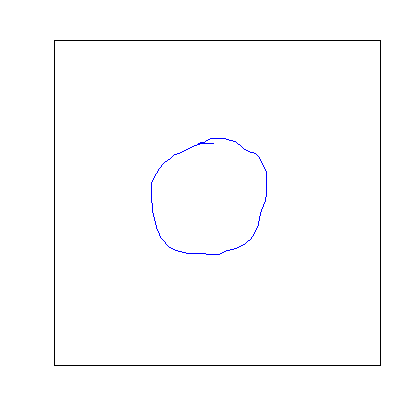
\includegraphics[width=\textwidth]{figs/0-1}
\caption{Zero-1}
\label{fig:figure1}
\end{minipage}
\hspace{0.5cm}
\begin{minipage}[b]{0.45\linewidth}
\centering
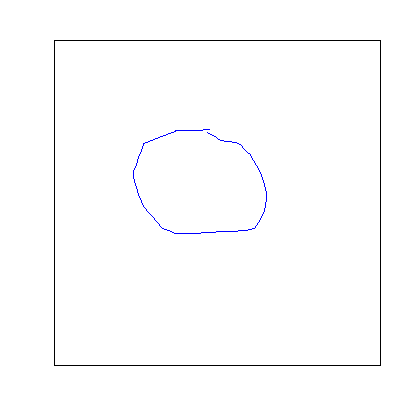
\includegraphics[width=\textwidth]{figs/0-2}
\caption{Zero-2}
\label{fig:figure2}
\end{minipage}
\end{figure}


%one
\begin{figure}[ht]
\begin{minipage}[b]{0.45\linewidth}
\centering

\includegraphics[width=\textwidth]{figs/1-1}
\caption{One-1}
\label{fig:figure1}
\end{minipage}
\hspace{0.5cm}
\begin{minipage}[b]{0.45\linewidth}
\centering

\includegraphics[width=\textwidth]{figs/1-2}
\caption{One-2}
\label{fig:figure2}
\end{minipage}
\end{figure}



%two
\begin{figure}[ht]
\begin{minipage}[b]{0.45\linewidth}
\centering

\includegraphics[width=\textwidth]{figs/2-1}
\caption{Two-1}
\label{fig:figure1}
\end{minipage}
\hspace{0.5cm}
\begin{minipage}[b]{0.45\linewidth}
\centering

\includegraphics[width=\textwidth]{figs/2-2}
\caption{Two-2}
\label{fig:figure2}
\end{minipage}
\end{figure}

%three
\begin{figure}[ht]
\begin{minipage}[b]{0.45\linewidth}
\centering
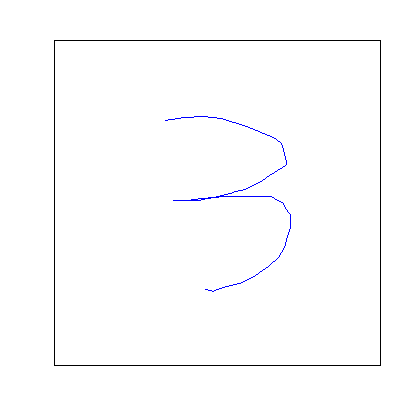
\includegraphics[width=\textwidth]{figs/3-1}
\caption{Three-1}
\label{fig:figure1}
\end{minipage}
\hspace{0.5cm}
\begin{minipage}[b]{0.45\linewidth}
\centering
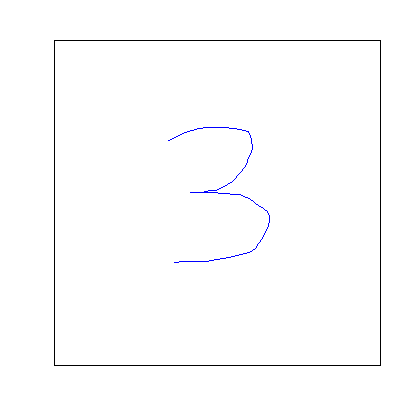
\includegraphics[width=\textwidth]{figs/3-2}
\caption{Three-2}
\label{fig:figure2}
\end{minipage}
\end{figure}

%four
\begin{figure}[ht]
\begin{minipage}[b]{0.45\linewidth}
\centering

\includegraphics[width=\textwidth]{figs/4-1}
\caption{Four-1}
\label{fig:figure1}
\end{minipage}
\hspace{0.5cm}
\begin{minipage}[b]{0.45\linewidth}
\centering
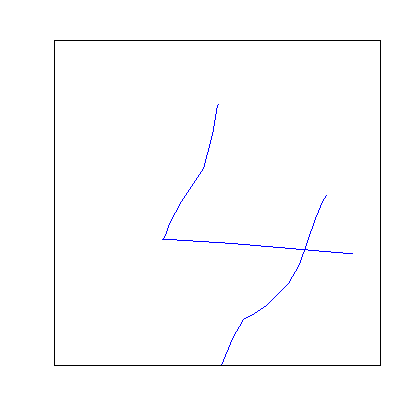
\includegraphics[width=\textwidth]{figs/4-2}
\caption{Four-2}
\label{fig:figure2}
\end{minipage}
\end{figure}

%five
\begin{figure}[ht]
\begin{minipage}[b]{0.45\linewidth}
\centering
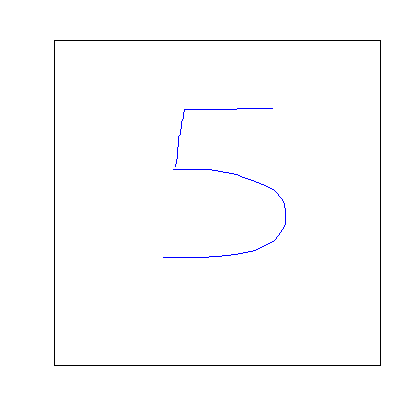
\includegraphics[width=\textwidth]{figs/5-1}
\caption{Five-1}
\label{fig:figure1}
\end{minipage}
\hspace{0.5cm}
\begin{minipage}[b]{0.45\linewidth}
\centering
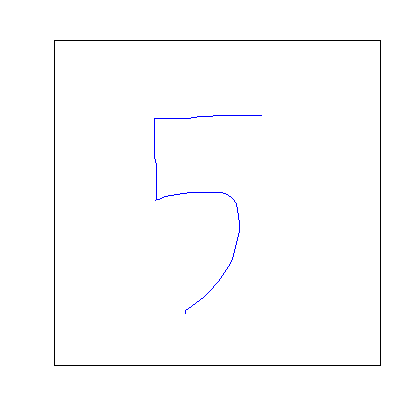
\includegraphics[width=\textwidth]{figs/5-2}
\caption{Five-2}
\label{fig:figure2}
\end{minipage}
\end{figure}

%six
\begin{figure}[ht]
\begin{minipage}[b]{0.45\linewidth}
\centering

\includegraphics[width=\textwidth]{figs/6-1}
\caption{Six-1}
\label{fig:figure1}
\end{minipage}
\hspace{0.5cm}
\begin{minipage}[b]{0.45\linewidth}
\centering
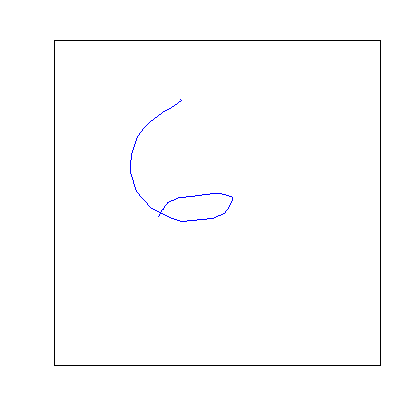
\includegraphics[width=\textwidth]{figs/6-2}
\caption{Six-2}
\label{fig:figure2}
\end{minipage}
\end{figure}

%seven
\begin{figure}[ht]
\begin{minipage}[b]{0.45\linewidth}
\centering

\includegraphics[width=\textwidth]{figs/7-1}
\caption{Seven-1}
\label{fig:figure1}
\end{minipage}
\hspace{0.5cm}
\begin{minipage}[b]{0.45\linewidth}
\centering

\includegraphics[width=\textwidth]{figs/7-2}
\caption{Seven-2}
\label{fig:figure2}
\end{minipage}
\end{figure}

%eight
\begin{figure}[ht]
\begin{minipage}[b]{0.45\linewidth}
\centering
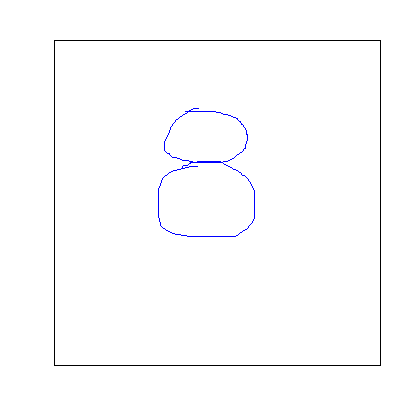
\includegraphics[width=\textwidth]{figs/8-1}
\caption{Eight-1}
\label{fig:figure1}
\end{minipage}
\hspace{0.5cm}
\begin{minipage}[b]{0.45\linewidth}
\centering
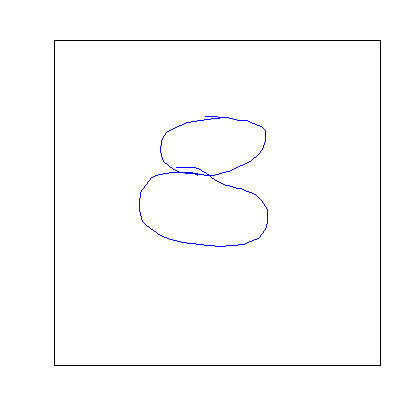
\includegraphics[width=\textwidth]{figs/8-2}
\caption{Eight-2}
\label{fig:figure2}
\end{minipage}
\end{figure}

%nine
\begin{figure}[ht]
\begin{minipage}[b]{0.45\linewidth}
\centering

\includegraphics[width=\textwidth]{figs/9-1}
\caption{Nine-1}
\label{fig:figure1}
\end{minipage}
\hspace{0.5cm}
\begin{minipage}[b]{0.45\linewidth}
\centering

\includegraphics[width=\textwidth]{figs/9-2}
\caption{Nine-2}
\label{fig:figure2}
\end{minipage}
\end{figure}

%plus
\begin{figure}[ht]
\begin{minipage}[b]{0.45\linewidth}
\centering
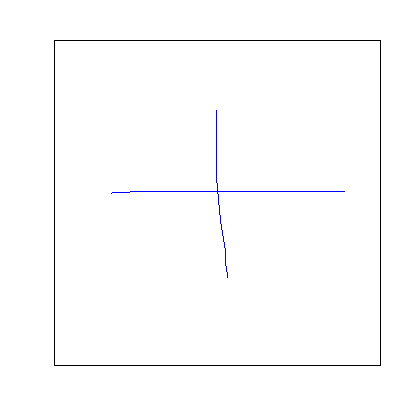
\includegraphics[width=\textwidth]{figs/+-1}
\caption{Plus-1}
\label{fig:figure1}
\end{minipage}
\hspace{0.5cm}
\begin{minipage}[b]{0.45\linewidth}
\centering
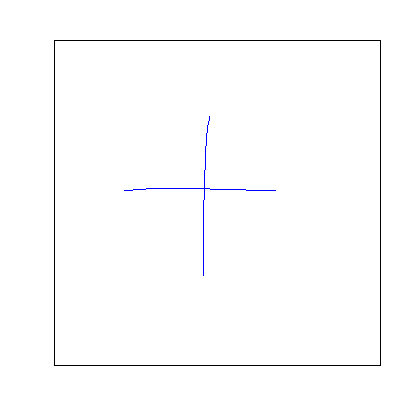
\includegraphics[width=\textwidth]{figs/+-2}
\caption{Plus-2}
\label{fig:figure2}
\end{minipage}
\end{figure}

%minus
\begin{figure}[ht]
\begin{minipage}[b]{0.45\linewidth}
\centering

\includegraphics[width=\textwidth]{figs/--1}
\caption{Minus-1}
\label{fig:figure1}
\end{minipage}
\hspace{0.5cm}
\begin{minipage}[b]{0.45\linewidth}
\centering

\includegraphics[width=\textwidth]{figs/--2}
\caption{Minus-2}
\label{fig:figure2}
\end{minipage}
\end{figure}

%div
\begin{figure}[ht]
\begin{minipage}[b]{0.45\linewidth}
\centering

\includegraphics[width=\textwidth]{figs/div-1}
\caption{Division-1}
\label{fig:figure1}
\end{minipage}
\hspace{0.5cm}
\begin{minipage}[b]{0.45\linewidth}
\centering

\includegraphics[width=\textwidth]{figs/div-2}
\caption{Division-2}
\label{fig:figure2}
\end{minipage}
\end{figure}

%multi
\begin{figure}[ht]
\begin{minipage}[b]{0.45\linewidth}
\centering
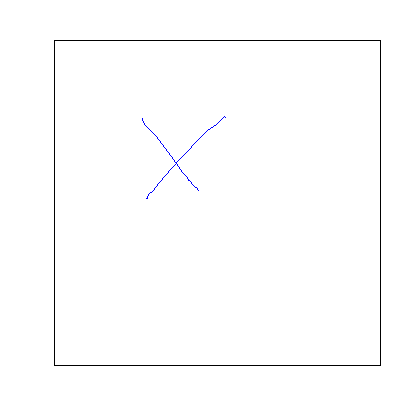
\includegraphics[width=\textwidth]{figs/x-1}
\caption{}
\label{fig:figure1}
\end{minipage}
\hspace{0.5cm}
\begin{minipage}[b]{0.45\linewidth}
\centering
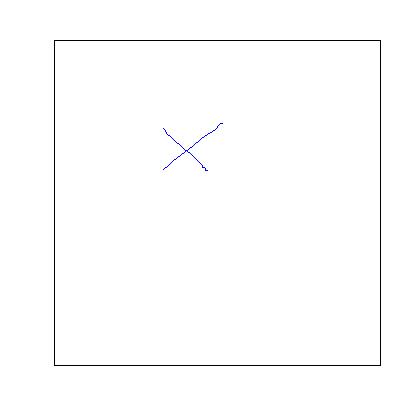
\includegraphics[width=\textwidth]{figs/x-2}
\caption{}
\label{fig:figure2}
\end{minipage}
\end{figure}


%equal
\begin{figure}[ht]
\begin{minipage}[b]{0.45\linewidth}
\centering
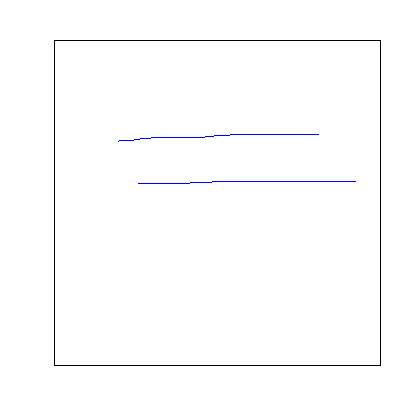
\includegraphics[width=\textwidth]{figs/=-1}
\caption{}
\label{fig:figure1}
\end{minipage}
\hspace{0.5cm}
\begin{minipage}[b]{0.45\linewidth}
\centering
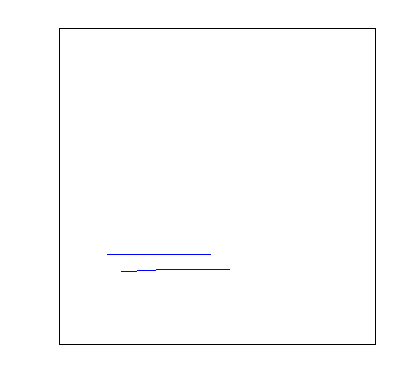
\includegraphics[width=\textwidth]{figs/=-2}
\caption{}
\label{fig:figure2}
\end{minipage}
\end{figure}

\end{document}